\chapter{Spazi Metrici}

\section{Preliminari}
% TODO definzione campo

\begin{definition}[Spazio Vettoriale]
	Siano $K$ un \textbf{campo} e $V$ un \textbf{insieme}. Si dice che \textbf{Spazio Vettoriale} sul campo $K$ se sono definite due operazioni:
	\begin{enumerate}
		\item \textbf{Somma}, operazione interna binaria
		\item \textbf{Prodotto per scalari} operazione esterna
	\end{enumerate}
	\begin{note}
		Questa definizione è stata riportata per ricordare il concetto, si consiglia la consultazione di un libro di Algebra Lineare per una definizione più precisa.
	\end{note}
\end{definition}

\begin{definition}[Spazio Metrico]
	\label{def:sp_metrico}
	Si dice Spazio Metrico $(X,d)$ un insieme $X$ non vuoto in cui sia definita una \textbf{distanza} (o \textbf{metrica}), vale a dire una funzione $d: X \times X \mapsto \R$ con le seguenti proprietà:
	\begin{enumerate}
		\item $d(x,y) \geq 0 \quad \forall x,y \in X$
		\item $d(x,y) = 0 \quad \forall x,y \in X \iff x=y$
		\item $d(x,y) = d(y,x) \quad \forall x,y \in X$ \quad(\textit{simmetria})
		\item $d(x,z) \leq d(x,y)+d(y,z) \quad \forall x,y,z\in X$ \quad(\textit{disuguaglianza triangolare})
	\end{enumerate}
\end{definition}

Unendo le due definizioni si giunge naturalmente a
\begin{definition}[Spazio Vettoriale Metrico]
	Uno Spazio Vettoriale Metrico è uno spazio vettoriale $V$ su cui è definito un prodotto scalare $<\cdot,\cdot·>$ definito positivo, la sua \textbf{metrica}.
	\begin{note}
		Analogamente si definisce il Sottospazio Vettoriale Metrico
	\end{note}
\end{definition}

\begin{definition}[Metrica Indotta]
	\label{def:metr_indotta}
	Siano $(X,d)$ spazio metrico e $S \subseteq X$ con $S \neq \emptyset$\\
	Allora $d_{|S} = d_{|S \times S}$ è una metrica su $S$, cioè la metrica $d_{|S}$ è la \textbf{metrica indotta}, definita come la \textbf{restrizione} della metrica $d$ ai soli elementi di $S$. Si definisce formalmente come
	$$\funcdef{d_{|S}}{S \times S}{\R}{(x,y)}{d(x,y)}$$
\end{definition}

\begin{definition}[Sottospazio Metrico]
	Siano $(X,d)$ spazio metrico e $S \subseteq X$ con $S \neq \emptyset$\\
	Allora $(S,d_{|S})$ con la \fullref{def:metr_indotta} è a sua volta Spazio Metrico ed è chiamato \textbf{Sottospazio Metrico di $(X,d)$}
	\begin{proof}
		La $d_{|S}$, essendo restrizione della metrica $d$, rispetta ancora tutti i punti della \fullref{def:sp_metrico}.
	\end{proof}
\end{definition}

\begin{proposition}
	\label{prop:subspace_condition}
	Sia $(V)$ uno spazio vettoriale metrico sul campo $K$ e sia $\emptyset \neq U \subseteq V$. Il sottoinsieme $U$ è un sottospazio vettoriale metrico se, e soltanto se, sono verificate le seguenti condizioni:
	\begin{enumerate}
		\item $\forall \mathbf{u}, \mathbf{u'} \in U \quad \mathbf{u} + \mathbf{u'} \in U$
		\item $\forall \lambda \in K,\; \forall \mathbf{u} \in U \quad \lambda \cdot \mathbf{u} \in U$
	\end{enumerate}
	\begin{proof}
		Non richiesta, analoga a quella per Spazi Vettoriali reperibile in un libro di Algebra Lineare
	\end{proof}
\end{proposition}

\begin{example}[Esempi di Metriche]
	\label{ex:metriche}
	Si dimostri che le seguenti funzioni sono distanze:
	\begin{note}
		Si noti che alcuni degli esempi sottostanti sono relativi a metriche trattate molto più avanti e dunque potrebbe essere conveniente ignorarli temporaneamente per tornare qui quando saranno stati fatti i successivi argomenti.
	\end{note}
	\begin{enumerate}
		\item $X=\R^2,\quad d(x,y) = d\bigl((x_1,x_2),(y_1,y_2)\bigr) = \sqrt{(y_1-x_1)^2+(y_2-x_2)^2}$ \hfill {\footnotesize\textbf{Metrica Euclidea in $\R^2$}}\\
			\begin{enumerate}[label=\arabic*]
				\item $d(x,y) \geq 0$ è verificata poiché l'argomento della radice è sempre positivo o al più nullo essendo una somma di quadrati, e la radice mantiene la positività.
				\item $d(x,y) = 0 \iff x = y$
					\begin{align*}
						d = 0 &\iff \sqrt{(y_1-x_1)^2+(y_2-x_2)^2} = 0\\
						&\iff (y_1-x_1)^2+(y_2-x_2)^2 = 0\\
						&\iff \begin{cases}
							(y_1-x_1)^2=0\\
							(y_2-x_2)^2=0\\
						\end{cases}\\
						&\iff
						\begin{cases}
							y_1=x_1\\
							y_2=x_2\\
						\end{cases}\\
						&\iff (x_1,x_2)=(y_1,y_2)
					\end{align*}
				\item $d(x,y) = d(y,x)$ invertendo le coordinate di $x$ con quelle di $y$ la somma non cambia, quindi la simmetria è rispettata
					$$d\bigl((x_1,x_2),(y_1,y_2)\bigr) \bigr) = \sqrt{(y_1-x_1)^2+(y_2-x_2)^2} = \sqrt{(y_2-x_2)^2+(y_1-x_1)^2} = d\bigl((y_1,y_2),(x_1,x_2)\bigr)$$
				\item $d(x,y) \leq d(x,z) + d(z,y)$ da \fullref{prop:dist_sp_norm}, la metrica indotta dalla norma (\fullref{def:norma}), applicata ad $\R^2$ è
					$$\norm{x - y} = \sqrt{(y_1-x_1)^2+(y_2-x_2)^2}$$
					che corrisponde alla metrica in oggetto. Dunque, grazie alle proprietà dell'operatore $\norm{\;\cdot\;}$ (nello specifico la \textit{disuguaglianza triangolare}), si ottiene
					$$d(x,y) = \norm{x-y} = \norm{(x-z) + (z-y)} \leq \norm{x-z} + \norm{z-y} = d(x,z) + d(z,y)$$
					\begin{center}
						\begin{tikzpicture}[scale=0.5]
						\draw (0,0) node[anchor=north east]{$x=(x_1,x_2)$}
							-- (4,4) node[anchor=south]{$y=(y_1,y_2)$}
							-- (4,0) node[anchor=north west]{$z=(z_1,z_2)$}
							-- cycle;
						\end{tikzpicture}
					\end{center}
			\end{enumerate}
		\item $X=\R,\quad d(x,y)=\abs{y-x}$ \hfill {\footnotesize\textbf{Metrica Euclidea in $\R$}}\\
			Analogo al primo esempio, nel dettaglio
			\begin{enumerate}[label=\arabic*.]
				\item $d(x,y) \geq 0$ per definizione valore assoluto
				\item $d(x,y) = 0 \iff x = y$ perché $\abs{\;\cdot\;} = 0 \iff \cdot\; = 0$ per definizione valore assoluto
				\item $d(x,y)=d(y,x)$ perché $\abs{x - y} = \abs{y - x}$ per definizione valore assoluto
				\item $d(x,y) \leq d(x,z) + d(z,y)$ in quanto
					$$d(x,y) = \abs{x-y} = \abs{x-z+z-y} \leq \abs{x-z} + \abs{z-y} = d(x,z) + d(z,y)$$
			\end{enumerate}
		\item $X=\R^n \;\; \text{con}\; x=(x_1,\ldots,x_n),\; y=(y_1,\ldots,y_n),\quad d(x,y)=\sqrt{\sum\limits_{i=1}^{n}{\left(y_i-x_i\right)}^2}$ \hfill {\footnotesize\textbf{Metrica Euclidea in $\R^n$}} \label{ex:dist_eucl}\\
			Analogo al primo esempio
		\item $X\ne \emptyset,\quad d(x,y)= \left\{\begin{matrix}0&&x=y\\1&&x \ne y\end{matrix}\right.$ \hfill {\footnotesize\textbf{Metrica Discreta}}\\
			\begin{enumerate}[label=\arabic*.]
				\item $d(x,y) \geq 0$ per definizione
				\item $d(x,y) = 0 \iff x = y$ per definizione
				\item $d(x,y)=d(y,x)$ per definizione (sia che $x = y$, sia che $x \neq y$)
				\item $d(x,y) \leq d(x,z) + d(z,y)$ perché $d(x,z) + d(z,y)$ può essere:
					\begin{itemize}
						\item $0$ se $x = y = z$, ma in questo caso anche $d(x,y) = 0$
						\item $1$ se $x = y \neq z$ o $x \neq y = z$, ma in questo caso $d(x,y) \leq 1$
						\item $2$ se $x \neq y \neq z$, quindi sicuramente $d(x,y) \leq d(x,z) + d(z,y)$
					\end{itemize}
			\end{enumerate}
		\item $X=\cntclass{0}(\realintervalclose{a}{b},\R)\;a,b\in\R,\;a<b \quad d_\infty(f,g) = \sup\limits_{x\in\realintervalclose{a}{b}}\abs{g(x)-f(x)}$ \hfill
			{\footnotesize
				\begin{tabular}{c}
					\textbf{Distanza della Convergenza Infinita}\\
					o\\
					\textbf{Distanza della Convergenza Uniforme}
				\end{tabular}
			}\label{ex:dim_dist_conv_unif}\\
			\begin{note}
				La metrica viene trattata in \fullref{def:conv_unif}
			\end{note}
			\begin{note}
				$X$ contiene infiniti elementi (funzioni)
			\end{note}
			\begin{center}
				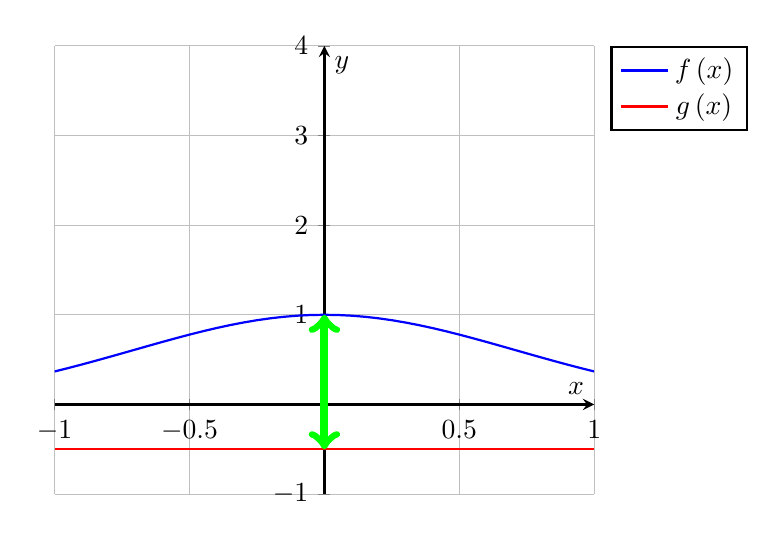
\begin{tikzpicture}[scale=1]
					\begin{axis}[
						xlabel={$x$},ylabel={$y$},
						axis lines=middle,
						samples=41,grid,thick,
						domain=-1:1,
						ymin=-1,ymax=4,
						legend pos=outer north east ]
						\addplot+[no marks] {e^-(abs(x*x))}; \addlegendentry{$f\left( x \right)$}
						\addplot+[no marks] {-0.5}; \addlegendentry{$g\left( x \right)$}
						\draw[<->,line width=1mm, color=green] (axis cs:0,-0.5) -- (axis cs:0,1);
					\end{axis}
				\end{tikzpicture}
			\end{center}
			\begin{enumerate}[label=\arabic*.]
				\item $d(x,y) \geq 0$ per definizione, il valore è sicuramente appartenente a $\realintervalclose{0}{+\infty}$, ma $+\infty$ non è un valore accettabile, in quanto la metrica è definita come funzione a valori in $\R$ e $+\infty \notin \R$. D'alto canto, si nota che $X$ è definito come l'insieme delle funzioni continue definite su un intervallo \textbf{chiuso e limitato} a valori in $\R$ ($\cntclass{0}(\realintervalclose{a}{b},\R)$). Questa definizione permette di applicare il \fullref{teo:weier} ed avere la certezza che esista $\sup$ finito.
				\item $d(x,y) = 0 \iff x = y$ per definizione, $d_\infty(f,g) = 0 \iff \sup\limits_{x\in\realintervalclose{a}{b}}\abs{g(x)-f(x)} = 0$, cioè se e solo se le due funzioni hanno lo stesso dominio e, per ogni punto di esso, la stessa immagine.
				\item $d(x,y)=d(y,x)$ semplicmente $d_{\infty}(f,g) = \sup\limits_{x\in\realintervalclose{a}{b}}\abs{f-g} = \sup\limits_{x\in\realintervalclose{a}{b}}\abs{g-f} = d_{\infty}(g,f)$
				\item $d(x,y) \leq d(x,z) + d(z,y)$ dalla disuguaglianza triangolare per $\abs{\;\cdot\;}$ si ottiene $\abs{g(x)-f(x)}\le\abs{g(x)-h(x)}+\abs{h(x)-f(x)}$. Applicando il sup la disuguaglianza resta vera.
			\end{enumerate}
			\begin{note}
				Si sottolinea che queste conclusioni sono valide finché $\realintervalclose{a}{b}$ chiuso e limitato, altrimenti non varrebbe più il \fullref{teo:weier} necessario per il punto 1. % TODO Serve un controesempio
			\end{note}
		\item $X=\R^2$, $d$ distanza Euclidea e $P$ punto arbitrario\\
			$\quad d_P(x,y)=
			\begin{cases}
				\begin{array}{ll}
					0 & \text{se } x = y\\
					d(x,P) + d(P,y) & \text{se } x \neq y
				\end{array}
			\end{cases}$ \hfill
			{\footnotesize
				\begin{tabular}{c}
					\textbf{Distanza di Parigi}\\
					o\\
					\textbf{Distanza Ferroviaria Francese}
				\end{tabular}
			} \label{ex:dist_parigi}\\
			\begin{enumerate}[label=\arabic*.]
				\item $d(x,y) \geq 0$ per definizione
				\item $d(x,y) = 0 \iff x = y$ per definizione
				\item $d(x,y)=d(y,x)$ essendo bassata sulla metrica Euclidea
				\item $d(x,y) \leq d(x,z) + d(z,y)$ essendo bassata sulla metrica Euclidea
			\end{enumerate}
		\item $X=\cntclass{0}(\realintervalclose{a}{b},\R)\;a,b\in\R,\;a<b \quad d_2(f,g) = \sqrt{\int_a^b\left[g(x)-f(x)\right]^2 \integrald{x}}$ \hfill {\footnotesize\textbf{Distanza Quadratica}}\\
		\label{ex:dim_dist_quadratica}
			\begin{note}
				La metrica viene trattata in \fullref{def:dist_quadratica}
			\end{note}
			\begin{enumerate}[label=\arabic*.]
				\item $d(x,y) \geq 0$ per definizione, essendo integrale di un valore positivo (quadrato) tra estremi ordinati ($a<b$ per ipotesi)
				\item $d(x,y) = 0 \iff x = y$ Per definizione della metrica, $d_2(f,g) = 0 \iff \sqrt{\int_a^b\left[g(x)-f(x)\right]^2 \integrald{x}} = 0$, cioè se e solo se le due funzioni hanno lo stesso dominio e, per ogni punto di esso, la stessa immagine.
				\item $d(x,y)=d(y,x)$ semplicmente $d_2(f,g) = \sqrt{\int_a^b\left[g(x)-f(x)\right]^2 \integrald{x}} = \sqrt{\int_a^b\left[f(x)-g(x)\right]^2 \integrald{x}} = d_2(g,f)$
				\item $d(x,y) \leq d(x,z) + d(z,y)$ ... % TODO Spiegare questo punto
			\end{enumerate}
	\end{enumerate}
\end{example}

\begin{definition}[Norma]
	\label{def:norma}
	Dato uno spazio vettoriale $V$ sul campo $\mathbb{K}$, si definisce \textbf{norma} una funzione $\norm{\cdot}:V\mapsto\R$ con le proprietà:
	\begin{enumerate}
		\item $\norm{x} \geq 0 \quad \forall x\in V$
		\item $\norm{x}=0 \iff x = 0 \quad \forall x\in V$
		\item $\norm{x+y} \leq \norm{x}+\norm{y} \quad \forall x,y\in V$
		\item $\norm{\lambda x} = \abs{\lambda} \cdot \norm{x} \quad \forall x\in V,\lambda\in\mathbb{K}$
	\end{enumerate}
	\begin{note}
		La funzione Norma associa dunque ad un vettore di qualsiasi dimensione uno scalare, fornendo (anche) una metrica per ordinare vettori tra loro.
	\end{note}
\end{definition}
\begin{definition}[Spazio Normato]
	Uno spazio normato è uno spazio vettoriale $V$ sul campo $\mathbb{K}$ \textbf{in cui è definita una norma}.
	\begin{note}
		Nel seguito verranno considerati esclusivamente spazi vettoriali su $\R$ o su $\C$, cioè $\mathbb{K} = \R$ o $\mathbb{K} = \C$
	\end{note}
\end{definition}

\begin{example}[Esempi di Spazi Normati]
	~
	\begin{enumerate}
		\item $\R$ con $\norm{x} = \abs{x}$
		\item $\C$ con $\norm{x} = \abs{x}$
		\item $\R^n$ con $\norm{x} = \sqrt{\sum\limits_{i=1}^{n}x_i^2}$
		\item $\cntclass{0}(\realintervalclose{0}{1};\R)$ con $\norm{f} = \sup\limits_{x \in \realintervalclose{0}{1}} \abs{f(x)}$
	\end{enumerate}
\end{example}

\begin{proposition}[Metrica Indotta da una Norma]
	\label{prop:dist_sp_norm}
	Sia $V$ uno spazio normato. Allora $(V,d)$ è uno spazio metrico con la distanza
	$$d(x,y) = \norm{y-x}$$
	ed inoltre la distanza così definita è:
	\begin{enumerate}
		\item Invariante per traslazioni:
			$$\forall x,y,z \in V,\; d(x,y) = d(x+z, y+z)$$
		\item Positivamente omogenea:
			$$\forall x,y \in V\: \text{e} \forall \lambda \in \R,\; d(\lambda x, \lambda y) = \abs{\lambda}d(x,y)$$
	\end{enumerate}
	\begin{proof}
		~
		\begin{enumerate}
			\item $d(x,y) = d(x+z, y+z) = \norm{y+z-x-z} = \norm{y-x} = d(x,y)$
			\item Con la proprietà 4 della \fullref{def:norma}
			$$d(\lambda x, \lambda y) = \norm{\lambda y - \lambda x} = \norm{\lambda (y - x)} = \abs{\lambda} \norm{y - x} = \abs{\lambda}d(x,y)$$
		\end{enumerate}
	\end{proof}
	\begin{note}
		Nel caso in cui $V = \R^n$, la metrica indotta è ovviamente la \textbf{Metrica Euclidea} di \hyperref[ex:dist_eucl]{\cref*{ex:metriche} (\nameref*{ex:metriche})}
		$$d(x,y) = \sqrt{\sum\limits_{i=1}^{n} (y_i-x_i)^2 }$$
	\end{note}
\end{proposition}

\begin{definition}[Metriche Equivalenti]
	Siano $d_1$ e $d_2$ due distanze sullo stesso insieme $X$.\\
	\begin{equation*}
		\begin{gathered}
			d_1 \text{ e } d_2 \text{ sono \textbf{equivalenti}}\\
			\bydef\\
			\exists c,C \in \realintervalopen{0}{+\infty}:\; \forall x,y \in X \quad c \cdot d_1(x,y) \leq d_2 (x,y) \leq C \cdot d_1 (x,y)
		\end{gathered}
	\end{equation*}
	Cioè se è sempre possibile "limitare" una metrica con l'altra (moltiplicata per un opportuno coefficiente). Questo implica che distanze infinite per una metrica devono esserlo anche per l'altra.
	\begin{note}
		Dato uno spazio metrico $(X,d)$, passare dalla distanza $d$ ad un'altra ad essa equivalente è concettualmente analogo ad un cambio di unità di misura. Come esempio si veda \fullref{ex:dist_eqiv}
	\end{note}
\end{definition}
\begin{example}
	La \hyperref[ex:dist_parigi]{Distanza Ferroviaria Francese da \cref*{ex:metriche} (\nameref*{ex:metriche})} e la \hyperref[ex:dist_eucl]{Metrica Euclidea da \cref*{ex:metriche} (\nameref*{ex:metriche})} non sono equivalenti
	% NOTE The \fullref command was not used on purpose to point this link straight to the right part of the aforementioned exercise
	\begin{solution}
		Operando in $\R$ e avendo un $n \in \N$:
		\begin{itemize}
			\item $P = 0$
			\item $x = n$
			\item $y = n+1$
		\end{itemize}
		Ora, per ogni $n$ la $d = 1$, mentre la $d_P = 2n+1$, dunque è impossibile trovare un $C \in \realintervalopen{0}{+\infty}$ (quindi finito) tale per cui
		$$d_P(x,y) \leq C \cdot d(x,y)$$
	\end{solution}
\end{example}
\begin{example}
	\label{ex:metr_equiv_R2}
	In $\R^2$, le distanze:
	\begin{align*}
		d_1(x,y) \;\; &= \;\; \abs{y_1 - x_1} + \abs{y_2 - x_2}\\
		d(x,y) \;\; &= \;\; \sqrt{(y_1 - x_1)^2 + (y_2 - x_2)^2}\\
		d_\infty(x,y) \;\; &= \;\; \max (\abs{y_1 - x_1}, \abs{y_2 - x_2})
	\end{align*}
	sono tutte equivalenti tra di loro.
\end{example}

\definition
\begin{definition}[Sfera]
	Sia $(X,d)$ uno spazio metrico e siano $x_0 \in X$, $r > 0$. Si dice \textbf{Sfera} (o \textbf{Bolla}, o ancora \textbf{Palla}) \textbf{Aperta} di centro $x_0$ e raggio $r$ l'insieme:
	$$B(x_0,r)=\brackets{x\in X : d(x,y)<r}$$
\end{definition}
\begin{observation}
	Se $r=0\Rightarrow B(x_0,r)=\emptyset$\\
	Se $r>0\Rightarrow x_0\in B(x_0,r)$
\end{observation}
\begin{exercise}
	Descrivere le sfere nelle distanze dell'\fullref{ex:metr_equiv_R2}.
	% TODO solution
\end{exercise}

\begin{definition}[Intorno]
	Sia $(X,d)$ uno spazio metrico e sia $x \in X$. \textbf{Intorno di} $\boldsymbol{x}$ è un qualunque sottoinsieme di $X$ che contenga una sfera aperta contentente $x$
\end{definition}

\example
In $\R$ con $d_E$, $B(x_0,r)$ è un intervallo simmetrico centrato in $x_0$
\example
In $\R^2$ con $d_E$, $B(x_0,r)$ è una un cerchio con centro in $x_0$
\example
In $\R^3$ con $d_E$, $B(x_0,r)$ è una sfera con centro in $x_0$
\example

% TODO le definizioni prima di questa nel capitolo 1
\begin{definition}
	\label{def:aperto}
	Sia $(X,d)$ spazio metrico, sia $A\subseteq X$. Si definisce
	$$A\text{ è \textbf{aperto}}\bydef A=\emptyset\quad\text{oppure}\quad A=\circdot{A}$$
\end{definition}

\begin{definition}
	\label{def:chiuso}
	Sia $(X,d)$ spazio metrico, sia $A\subseteq X$. Si definisce
	$$A\text{ è \textbf{chiuso}}\bydef A=\emptyset\quad\text{oppure}\quad A=\bar{A}$$
\end{definition}

\definition
Siano $(X,d_1)$ e $(X,d_2)$ spazi metrici. $d_1$ e $d_2$ sono equivalenti $\leftrightharpoons \exists c,C\in\R, c_1>0, c_2>0$ t.c:
$$ \forall x,y \in X\quad cd_1(x,y)\le d_2(x,y)\le Cd_1(x,y) $$

\definition
Un insieme è finito se il numero dei suoi elementi è finito
\definition
Un insieme è infinito se non è finito
\definition
Sia $(X,d)$s.m., $A\subseteq X$, $A\ne \emptyset$ si definisce diametro di A: $$diam(A)=\sup\limits_{x,y\in A}d(x,y)$$
\definition
$A$ è limitato $\leftrightharpoons diam(A)$ è finito ($\in\R$)
\definition
$A$ è illimitato $\leftrightharpoons diam(A)$ è infinito ($=\infty$)
\example
...\\
...\\
...\\
..\\
....\\
\observation
Ogni insieme finito è limitato e ogni insieme illimitato è infinito. Non valgono i viceversa.
\example
.....\\
....\\
.....\\
......\\
.....\\
....\\


\section{Successioni e Completezza}
\begin{definition}
	% TODO Definizione successione
\end{definition}
\begin{definition}
	% TODO Successione limitata
\end{definition}
\begin{definition}
	% TODO Successione convergente
\end{definition}
\begin{proposition}
	\label{prop:succ_conv_lim}
	Data la successione $x: \N \mapsto X$ di elementi dello spazio metrico $(X,d)$ e dato $x_\infty\in X$:
	$$\lim\limits_{n\rightarrow+\infty}x_n=x_\infty\iff\forall\varepsilon > 0\;\;\exists\nu\in\N:\quad\forall n>\nu\;\;d(x_n,x_\infty)<\varepsilon$$
	\begin{proof}
		% TODO dimostrazione
	\end{proof}
\end{proposition}
\subsection{Insiemi Compatti}
\begin{definition}[Insieme Compatto]
	\label{def:compatto}
	Sia $(X,d)$ uno spazio metrico e sia $A \subseteq X$. $A$ è compatto se e solo se ogni successione di elementi di $A$ ammette una sottosuccessione avente limite in $A$.
	\begin{note}
		Questa è la definizione di \textbf{Compattezza per Successioni}, in spazi più generali può essere necessario utilizzare una definizione più debole che, nel caso degli spazi metrici, coincide con la precedente.
	\end{note}
\end{definition}
\begin{exercise}
	\label{ex:unione_compatti}
	Sia $(X,d)$ uno spazio metrico. Siano $K_1$ e $K_2$ due sottoinsiemi compatti di $X$. Allora $K_1 \cup K_2$ è compatto
	\begin{solution}
		Posto $K = K_1 \cup K_2$, per definizione di \textbf{unione}, ogni elemento di $K$ è in $K_1$ o $K_2$.
		Visto che, per ipotesi, $K_1$ e $K_2$ sono compatti, sappiamo che ogni successione in uno dei due avrà una sottosuccessione convergente nello stesso insieme. A questo punto possiamo concludere che ogni successione in $K$ ammetterà una sottosuccessione convergente ad un elemento $x_\infty \in K_1$ oppure $x_\infty \in K_2 \implies x_\infty \in K$
	\end{solution}
\end{exercise}
\begin{exercise}
	\label{ex:dist_eqiv}
	% TODO copiare esercizio 2.42
\end{exercise}

\section{Limiti e Continuità}
\begin{definition}
	Siano $(X,d_x)$ e $(Y,d_y)$ spazi metrici, $A\subseteq{X}$,$x_0$ di accumulazione per $A$, $f:A\rightarrow{Y}$ una funzione e $l\in{Y}$ \\
	$\lim\limits_{x \rightarrow x_0} = l \bydef \forall{\varepsilon},\exists\delta : \forall{x}\in A : d_x(x,x_0)<\delta e x\ne{x_0} : d_y(f(x),l)<\varepsilon$
\end{definition}

\begin{proposition}
	Siano $(X,d_x)$ e $(Y,d_y)$ spazi metrici, $A\subseteq{X}$,$x_0$ di accumulazione per $A$, $f:A\rightarrow{Y}$ una funzione e $l'\in{Y}$,$l''\in{Y}$
\end{proposition}

\begin{definition}[Funzione Continua]
	\label{def:funz_cont}
	Siano $(X,d_X)$ e $(Y,d_Y)$ spazi metrici e sia $f: A \mapsto Y$ con $A \subseteq X$ e sia $x_0 \in A$
	\begin{equation*}
		\begin{gathered}
			f \text{ è \textbf{continua} in } x_0 \iff\\
			\forall \varepsilon > 0\;\;\exists \delta > 0:\quad \forall x \in A \text{ con } d_X(x,x_0)<\delta \text{ vale } d_Y \bigl(f(x),f(x_0)\bigr) < \varepsilon
		\end{gathered}
	\end{equation*}

	\begin{center}
		$f$ è \textbf{continua} in $A\bydef$\\
		$f$ è continua \textbf{in ogni punto} di $A$
	\end{center}
	\begin{note}
		Non andrebbe detto semplicemente $f$ \textit{è continua} perché la continuità dipende in modo essenziale dall'insieme di punti su cui la funzione viene considerata. In assenza di ulteriori specificazioni, spesso si sottointende che l'insieme in esame è l'intero dominio della funzione.
	\end{note}
	\begin{note}
		Ha senso valutare la continuità di una funzione esclusivamente nell'insieme in cui è definita. Quindi una frase come:\\
		\textit{la funzione} $x \mapsto \frac{1}{x}$ \textit{è discontinua in} $0$,\\
		non è (a rigore) sensata. Andrebbe riformulata come:\\
		\textit{la funzione} $x \mapsto \frac{1}{x}$ \textit{non può essere estesa ad una funzione definita e continua anche in} $0$.
	\end{note}
	\begin{note}
		La continuità di una funzione dipende in modo esssenziale anche dalla distanza adottata, tuttavia è prassi sottointendere questa precisazione, soprattutto per funzioni $\R^n \mapsto \R^n$, se la distanza adottata è quella Euclidea.
	\end{note}
\end{definition}

\begin{theorem}[Teorema generale di Weierstrass]
	\label{teo:weier_generale}
	Siano $(X,d_X)$ e $(Y,d_Y)$ spazi metrici e sia $f:K \mapsto Y$ con $K \subseteq X$.
	$$\left.\begin{array}{ll}
		K\;\text{compatto} \\
		f\;\text{continua su } K
		\end{array} \quad\right\} \implies f(K)\;\text{compatto}$$
	\begin{proof}
		Siano le successioni
		\begin{itemize}
			\item $y: \N \mapsto Y$ tale che $y_n \in f(K) \;\forall n \in \N$, cioè $\forall n \in \N\;\exists x_n \in K: f(x_n) = y_n$
			\item $x: \N \mapsto X$ tale che $x_n \in K\;\forall n \in \N$
		\end{itemize}
		\begin{note}
			Abbiamo una successione che, attraverso la $f$ (non direttamente: le successioni non sono $X \mapsto Y$!), associa indirettamente valori in $K \subseteq X$ a valori in $f(K) \subseteq Y$
		\end{note}
		La successione $x$ ammette una sottosuccessione $x_{n_k}$ convergente ad un elemento $\overline{x} \in K$ dalla \fullref{def:compatto}, avendo $K$ compatto per ipotesi, ed essendo $x$ a valori in $K$.\\
		Data la continuità di $f$ in $K$, abbiamo $y_{n_k} = f(x_{n_k}) \in f(K)$, ma essendo $x_{n_k}$ convergente ad $\overline{x}$, anche $y_{n_k}$ converge, verificando così la definizione di spazio Compatto.
	\end{proof}
	\begin{proof} (Alternativa)\\
		La successione $x$ ammette una sottosuccessione $x_{n_k}$ convergente ad un elemento $\overline{x} \in K$, dunque da \fullref{prop:succ_conv_lim}:
		$$\lim\limits_{n\rightarrow+\infty}x_n=x_*\iff\forall\eta > 0\;\;\exists\nu\in\N:\quad\forall n>\nu\;\;d(x_n,x_*)<\eta$$
		Dalla \fullref{def:funz_cont} e sapendo che $f(x)$ è continua, sappiamo che:
		$$\forall\varepsilon > 0\;\;\exists\delta > 0:\quad\forall x \in K\;\;d_X (x,x_*)<\delta\;\;d_Y \bigl(f(x_n),f(x_*)\bigr)<\varepsilon$$
		Unisco ora le due definizioni:
		$$\forall \varepsilon > 0\;\;\exists \nu \in \N:\quad \forall n > \nu\;\;d_Y \bigl(f(x_n),f(x_*)\bigr)<\varepsilon$$
		Che equivale, per come è definita $y_n$, a
		$$\lim\limits_{n\rightarrow +\infty}y_n = y_*$$
		Cioè la definizione di successione convergente. Ho dunque individuato una sottosuccessione convergente per ogni successione in $f(K)$, verificando così la definizione di spazio Compatto.
	\end{proof}
\end{theorem}

\subsection{Uniforme Continuità}
\begin{definition}[Funzione Uniformemente Continua]
	\label{def:unif_cont}
	Siano $(X,d_X)$ e $(Y,d_Y)$ spazi metrici. Sia $f:A \mapsto Y$ con $A \subseteq X$.
	\begin{center}
		$f$ è \textbf{uniformemente continua} in $A$\\
		$\bydef$\\
		$\forall \epsilon > 0 \quad \exists \delta > 0 \text{ tale che } \forall x,x_0 \in A \text{ con } d_X(x,x_0) < \delta \quad \text{vale } d_Y\bigl(f(x),f(x_0)\bigr) < \epsilon$
	\end{center}
\end{definition}
\begin{exercise}
	\label{ex:cont_unif_cont_comparision}
	Confrontare la \fullref{prop:AAA} con la \fullref{def:unif_cont}
	% TODO Proposizione 3.12 dal libro e soluzione
\end{exercise}
\begin{proposition}
	\label{prop:if_unif_cont_then_conf}
	Siano $(X,d_X)$ e $(Y,d_Y)$ spazi metrici. Sia $f:A \mapsto Y$ con $A \subseteq X$. Se $f$ è \textbf{uniformemente continua} in $A$, allora $f$ è \textbf{continua} in $A$.
	\begin{proof}
		Deriva da \fullref{ex:cont_unif_cont_comparision}
	\end{proof}
\end{proposition}
\subsection{Lipschitzianità}
\begin{definition}[Funzione Lipschitziana]
	\label{def:lips}
	Siano:
	\begin{itemize}
		\item $(X,d_X)$, $(Y,d_Y)$ spazi metrici
		\item $A \subseteq X$
		\item $f:A \mapsto Y$
	\end{itemize}
	Allora
	\begin{center}
		$f$ è \textbf{Lipschitziana}
	\end{center}
	\begin{equation*}\label{eq1}
		\begin{gathered}
			\leftrightharpoons \\
			\exists L > 0:\; \forall x_1,\,x_2 \in X,\;d_Y\bigl(f(x_1),f(x_2)\bigr)\leq L \cdot d_X(x_1,x_2)
		\end{gathered}
	\end{equation*}
\end{definition}

\section{Il Teorema delle Contrazioni}
\begin{definition}[Contrazione]
	\label{def:contrazione}
	Sia $(X, d)$ uno spazio metrico. Si dice contrazione una funzione T: $X \mapsto X$ soddisfacente a:
	\begin{align}
		\label{eq:def_contrazione}
		\exists K \in [0, 1[\;\text{tale che}\;\forall x',x''\in X\;\text{vale}\\
		d_X(T(x''), T(x')) \le K \cdot d_X(x'', x').
	\end{align}


	Una contrazione è quindi una funzione con insieme di partenza e di arrivo coincidenti e
	Lipschitziana con costante di Lipschitz strettamente minore di 1.
	E generalmente inutile considerare contrazioni definite tra spazi diversi. Data una funzione
	$T: X\rightarrow Y$ Lipschitziana, è sempre possibile riscalare la distanza in uno dei due spazi X o Y
	per ottenere una costante di Lipschitz minore di 1.
	\begin{note}
		D'ora in poi si utilizzerà spesso la notazione $Tx$ per intendere $T(x)$
	\end{note}
\end{definition}

ESEMPI:\\
\begin{enumerate}
	\item $f: \R \rightarrow \R$ data da $f(x) = \frac{x}{2}$. $f$ è una contrazione.
	\item $f: [0,2] \rightarrow [0,2]$ data da $f(x) = 1+\frac{x}{2}. f$ è una contrazione
	\item $f: \R^2 \rightarrow \R^2$ data da $f(x,y)=\begin{bmatrix} \frac{1}{3}&&0\\0&&\frac{1}{5}\end{bmatrix}$ è una contrazione
\end{enumerate}

\proposition
Sia $(X, d)$ uno spazio metrico, siano $f,g:X\rightarrow X$ due contrazioni in $X \Rightarrow f\circ g$ è una contrazione
\begin{proof}
	Sappiamo che\\
	$$\forall x',x''\in X, d(fx'', fx')\le K_fd(x'', x').$$
	$$\forall x',x''\in X, d(gx'', gx')\le K_gd(x'', x').$$
	$f\circ g=f(g(x))$, quindi presi $x',x''\in X$ si ha che: $$d(fg(x''), fg(x'))\le K_fd(g(x''), g(x'))\le K_fK_gd(x'',x').$$
\end{proof}

\proposition
Sia $f \in C1(R^n;R^n)$. Se $\exists k \in [0, 1[$ tale che $\forall x \in \R^n$ vale $\norm{Df(x)}  < k$, allora $f$ è una contrazione.

\begin{theorem}[Teorema delle Contrazioni]
	\label{teo:contrazioni}
	Sia $(X, d)$ uno spazio metrico completo in cui è definita una contrazione
	$T: X \rightarrow X$. Allora esiste un unico punto fisso di $T$ in $X$.
	\begin{proof}
		Costruisco una successione di elementi di $X$ nel seguente modo:\\
		scelgo $x_0\in X$,\\
		$x_1 = Tx_0$\\
		$x_2 = Tx_1$\\\\
		...\\
		$x_n = Tx_{n-1}$\\
		La successione ${x_n: n \in N }$ così costruita è una successione di Cauchy. Infatti, presi $n, m \in N$ con $m > n$ si ha:
		$$d(x_{m},x_{n}) = d(Tx_{m-1},x_{n-1}) \le Kd(x_{m-1},x_{n-1})=$$
		$$=Kd(x_{m-1},x_{n-1}) = Kd(Tx_{m-2},x_{n-2}) \le K^2d(x_{m-2},x_{n-2})=$$
		$$=...=$$
		$$=...=K^nd(x_{m-n},x_{0})\le$$
		$$\le K^{n}\sum\limits_0^{m-n+1}(d(x_{m-n-i},x_{m-n-i-1}))=$$
		$$\le \sum\limits_0^{m-n+1}(d(Tx_{m-n-i-1},Tx_{m-n-i-2}))$$
		per ogni termine di questa sommatoria si può applicare lo stesso ragionamento
		$$\le K^{n}\sum\limits_0^{m-n+1}(K^{m-n-2}d(Tx_{0},x_{0}))=$$
		$$\le K^{n}d(Tx_{0},x_{0})\sum\limits_0^{m-n+1}K^{m-n-2}=K^n\frac{1-K^{m-n-1}}{1-K}d(Tx_{0},x_{0}) \le \frac{K^n}{1-K}d(Tx_{0},x_{0})$$
		Ho quindi trovato che $d(x_{m},x_{n})\le\frac{K^n}{1-K}d(Tx_{0},x_{0})$\\
		L’ultima espressione ottenuta può essere resa arbitrariamente piccola (in modulo) pur di
		prendere $n$, e quindi anche $m$, sufficientemente elevato. La completezza di $X$ implica quindi
		che esiste il limite $\lim\limits_{n\rightarrow +\infty}xn$. Sia $x^*$ questo limite. $x^*$ è un punto fisso per $T$. Infatti, grazie
		alla continuità di $T$:
		$$T(x^*)=T{\lim\limits_{n\rightarrow +\infty}xn}$$
	\end{proof}
\end{theorem}

\begin{definition}[Funzione Iterata]
	\label{def:iterata}
	Data $F:X\mapsto X$, si dice funzione iterata $n$ volte di $F$ la $F^n$ che corrisponde all'applicazione $n$ volte di $F$ su sè stessa. Formalmente:
	$$f^{n+1} = f \circ f^n \quad \forall n \in \N\setminus\brackets{0}$$
	Se $n = 0$, per definizione, $f^0 = \mathrm{Id}_X$ con $\mathrm{Id}_X$ funzione identità su $X$
\end{definition}

\begin{theorem}[Teorema dell'Iterata Contrazione]
	\label{teo:iterata_contraz}
	Sia $(X,d_X)$ uno spazio metrico completo e sia $T:X\mapsto X : \exists n \in \N, T^n$ \textbf{iterata} è contrazione.\\
	Allora $T$ ammette un unico punto fisso in $X$
	\begin{note}
		La $n$ non è univocamente definita e non potrebbe esserlo. Se infatti $T^n$ è contrazione, allora anche $T^{2n},\, T^{3n},\, \cdots,\, T^{\alpha n}$ lo sono.
	\end{note}
	\begin{proof}
		Per il \fullref{teo:contrazioni} esiste un unico punto fisso $x_* \in X$ per $T^n$, quindi
		$$T^nx_* = x_*$$
		applicando $T$ ad entrambi i membri
		$$T(T^{n}x_*) = Tx_*$$
		e per la \fullref{def:iterata}
		$$T(T^{n}x_*) = T^n(Tx_*) = Tx_*$$
		Dunque $Tx_*$ è punto fisso della $T^n$. Avevamo però già trovato che $x_*$ era punto fisso della $T^n$ e, per il \fullref{teo:contrazioni}, può esistere un unico punto fisso. Ciò permette di concludere che $Tx_* = x_*$
	\end{proof}
\end{theorem}

\section{Funzioni a Valori in \texorpdfstring{$\protect \R$}{R}}
%TODO This section is a placeholder